\documentclass[11pt, a4paper, twoside, openright]{article} 
\usepackage{graphicx,color}
\usepackage{amssymb, amsmath, array}
\usepackage{hyperref}

\usepackage{wrapfig}
\begin{document}
% Example of title page for the projects carried out within DEDIS
% Copied from lasec 

% Simply include it in your mastex tex file: 
%        % Example of title page for the projects carried out within DEDIS
% Copied from lasec 

% Simply include it in your mastex tex file: 
%        % Example of title page for the projects carried out within DEDIS
% Copied from lasec 

% Simply include it in your mastex tex file: 
%        \input{cover}


% Updated October 2016


\newcommand{\logoepfl}[0]{
  \begin{center}
    
\includegraphics[width=4cm]{logo_epfl_coul.eps}
  \end{center}
  \vspace{0.3cm}
  \hrule
}
\newcommand{\project}[1]{
  \begin{center}
    \large{#1}
  \end{center}
  \vspace{1cm}
}
\newcommand{\department}[1]{
  \begin{center}
    \large{#1}
  \end{center}
}
\newcommand{\lab}[1]{
  \begin{center}
    \large{#1}
  \end{center}
}
\newcommand{\supervisor}[3]{
  \begin{center}
    \begin{normalsize}{
        \bf #1}\\#2\\#3
    \end{normalsize}
  \end{center}
}
\renewcommand{\author}[1]{
  \begin{center}
    \Large{#1}
  \end{center}
  \vspace{0.5cm}
}
\renewcommand{\title}[1]{
  \vspace{3cm}
  \begin{center}
    \huge{#1}
  \end{center}
  \vspace{1.7cm}
}
\renewcommand{\date}[2]{
  \begin{center}
    \normalsize{#1 #2}
  \end{center}
  \vspace{0.5cm}
}


\thispagestyle{empty}


% begin title page
  \logoepfl
  
  \title{Collective Certificate Management}
  
  \author{Robin Berguerand}
  \department{School of Computer and Communication Sciences}
  \lab{Decentralized and Distributed Systems lab}
  \project{Bachelor Project}
  
  \date{January}{2018}

  \begin{center}
    \begin{tabular}{cc}
      \begin{tabular}{p{4.0cm}}
        \supervisor{Responsible}{Prof. Bryan Ford}{EPFL / DEDIS}
      \end{tabular}&
      \begin{tabular}{p{4.0cm}}
        \supervisor{Supervisor}{Philipp Jovanovic / Linus Gasser}{EPFL / DEDIS}
      \end{tabular}
    \end{tabular}
  \end{center}

% end title page




% Updated October 2016


\newcommand{\logoepfl}[0]{
  \begin{center}
    
\includegraphics[width=4cm]{logo_epfl_coul.eps}
  \end{center}
  \vspace{0.3cm}
  \hrule
}
\newcommand{\project}[1]{
  \begin{center}
    \large{#1}
  \end{center}
  \vspace{1cm}
}
\newcommand{\department}[1]{
  \begin{center}
    \large{#1}
  \end{center}
}
\newcommand{\lab}[1]{
  \begin{center}
    \large{#1}
  \end{center}
}
\newcommand{\supervisor}[3]{
  \begin{center}
    \begin{normalsize}{
        \bf #1}\\#2\\#3
    \end{normalsize}
  \end{center}
}
\renewcommand{\author}[1]{
  \begin{center}
    \Large{#1}
  \end{center}
  \vspace{0.5cm}
}
\renewcommand{\title}[1]{
  \vspace{3cm}
  \begin{center}
    \huge{#1}
  \end{center}
  \vspace{1.7cm}
}
\renewcommand{\date}[2]{
  \begin{center}
    \normalsize{#1 #2}
  \end{center}
  \vspace{0.5cm}
}


\thispagestyle{empty}


% begin title page
  \logoepfl
  
  \title{Collective Certificate Management}
  
  \author{Robin Berguerand}
  \department{School of Computer and Communication Sciences}
  \lab{Decentralized and Distributed Systems lab}
  \project{Bachelor Project}
  
  \date{January}{2018}

  \begin{center}
    \begin{tabular}{cc}
      \begin{tabular}{p{4.0cm}}
        \supervisor{Responsible}{Prof. Bryan Ford}{EPFL / DEDIS}
      \end{tabular}&
      \begin{tabular}{p{4.0cm}}
        \supervisor{Supervisor}{Philipp Jovanovic / Linus Gasser}{EPFL / DEDIS}
      \end{tabular}
    \end{tabular}
  \end{center}

% end title page




% Updated October 2016


\newcommand{\logoepfl}[0]{
  \begin{center}
    
\includegraphics[width=4cm]{logo_epfl_coul.eps}
  \end{center}
  \vspace{0.3cm}
  \hrule
}
\newcommand{\project}[1]{
  \begin{center}
    \large{#1}
  \end{center}
  \vspace{1cm}
}
\newcommand{\department}[1]{
  \begin{center}
    \large{#1}
  \end{center}
}
\newcommand{\lab}[1]{
  \begin{center}
    \large{#1}
  \end{center}
}
\newcommand{\supervisor}[3]{
  \begin{center}
    \begin{normalsize}{
        \bf #1}\\#2\\#3
    \end{normalsize}
  \end{center}
}
\renewcommand{\author}[1]{
  \begin{center}
    \Large{#1}
  \end{center}
  \vspace{0.5cm}
}
\renewcommand{\title}[1]{
  \vspace{3cm}
  \begin{center}
    \huge{#1}
  \end{center}
  \vspace{1.7cm}
}
\renewcommand{\date}[2]{
  \begin{center}
    \normalsize{#1 #2}
  \end{center}
  \vspace{0.5cm}
}


\thispagestyle{empty}


% begin title page
  \logoepfl
  
  \title{Collective Certificate Management}
  
  \author{Robin Berguerand}
  \department{School of Computer and Communication Sciences}
  \lab{Decentralized and Distributed Systems lab}
  \project{Bachelor Project}
  
  \date{January}{2018}

  \begin{center}
    \begin{tabular}{cc}
      \begin{tabular}{p{4.0cm}}
        \supervisor{Responsible}{Prof. Bryan Ford}{EPFL / DEDIS}
      \end{tabular}&
      \begin{tabular}{p{4.0cm}}
        \supervisor{Supervisor}{Philipp Jovanovic / Linus Gasser}{EPFL / DEDIS}
      \end{tabular}
    \end{tabular}
  \end{center}

% end title page


\tableofcontents
\section{Introduction}
\paragraph{}In today's Internet, most of the communication needs to be encrypted to ensure confidentiality and integrity of the data. Before a secured communication channel can be open between two devices (for example, between Alice and Bob), they need to exchange their public keys. Those permits to Alice to send encrypted messages to Bob ensuring that he will be the only one who can decrypt it and vice versa. The problem with this exchange is that Bob needs to be certain that the public key that he receives is indeed Alice key. For example, a man-in-the-middle attacker can usurp the identity of Alice and sent his public key to Bob. Because Bob believes that he gets Alice key, he will send her confidential encrypted messages using the attacker key. Thus, the attacker will be able to read those messages using his private key.
Those attack could became very critical if a secured communication should be establish between an client and certain web server like ebanking service or commercial website.   
\paragraph{}
One solution that has been developed to prevent this type of attack was to create Certification Authorities (CAs). Those entities deliver certificate that permit to prove that a key belong to the appropriate device. Typically, a web server owner will request a certificate from a CA so that he can proves to its clients that they use the right public key to communicate with him. Therefore, a certificate contains at least the identity of the issuers, its public key and the validities dates of the certificate. The CA verifies the identity of the issuers (using divers mechanism depending the CA) and sign the certificate using its private key to prove its authenticity. By now, a browser that want to establish a secure channel (typically using HTTPS) with a web server firstly get its certificate. The browser can then verify the signature of the certificate using public key of the CA.  
However, this creates a chicken-and-egg problem: How do we recognize that we get right CAs public key? The solution to this issues is to store the public key of multiple CAs initially on the web browser.
\paragraph{}
This configuration raises new issues. How do we ensure, that a particular CA is trustworthy? A CA could be attacked and his private key could be stolen. Therefore, the attacker could be able to deliver false certificates an impersonate some website. Then, encrypted communication can be stolen which could cause major issue for some application.  
Moreover,a Certificate Authorities could be improperly configured and thus deliver inappropriate certificate. Hence, an user could accidentally or maliciously request a certificate for a domain that he doesn't own. 
\paragraph{}
Therefore, because of those problem, Certificate Authorities are criticals points in the Internet security.
This project present some solution that can reinforce the actual security level of the certificate process. We will use ideas described in a research paper named "Keeping "Honest or Bust" Decentralized Witness Co-signing" \cite{1} co-written by researchers of the EPFL and the Yale University. It states that instead of centralised entity like CAs, certificates could be manage by a decentralised protocol involving multiple entities. In this configuration, the certificate can be signed by multiple entities and then being considered as more trustworthy.
\subsection{Goals and Motivation}
The goal of this project is to develop a new decentralized infrastructure that will permit a more secure management of certificates and as explained in the introduction, avoid false certificates. This infrastructure need to be maintained and manipulated by multiple devices. Those devices could be for example CA servers or any other devices. 
\subsubsection{A Decentralized Infrastructure}
Implement such infrastructure requires to find a protocol that can permit to multiple peer to communicate and thus take decisions together. The group need to be able to decide if a certificate is valid or not and make the appropriate manipulation in accordance of their choice. If a certificate is valid it should be stored in the infrastructure.
The improvements of a decentralized infrastructure are multiple:
\paragraph{}
Every connected device on the infrastructure (or a majority of them) should approve the correctness of a certificate before it can be considered valid and then stored. Therefore, any wrong certificate can be detected by some of the device and thus invalidated. Thus, the authenticity and the correctness of a certificate is improved because it was controlled by multiple entity and not only one.
\paragraph{}
The complete system will be complex to be taken down by any attack because an attacker would need to hack all (or at least a majority) of the devices. Hence, the attacker needs to find vulnerabilities in many device which may take an extensive amount of time. Thus, the attack can probably be detected on time, and solutions to prevent it could be found.
\subsubsection{Automatic and Free Certificate}
One of the other goals of the project is to reduce the difficulties to a domain owner to obtain a certificate to his web server. We want to create a one line command that can request a certificate from a CA without any manipulation coming from a client. Moreover, this acquirement should be free and available at any time. As a motivation, it is known that getting an SSL certificate to pass his website from an HTTP to an HTTPS protocol can be onerous and complicated. This project could then help some domains owner to secure their website and thus improve the whole Internet security level. Logically, even if it is easier to request a certificate, it should remain totally secure.
\subsubsection{Compatibility}
\paragraph{}The certificate protocol is now greatly established on the Internet. Thus, it would be hard to change the whole system. Therefore, this new infrastructure should be compatible with current protocol to be easily deployed. One of the project's goal will be to add a new security protection on the top of yet existing mechanism to make it even more secure.     
\subsubsection{Framework}
\paragraph{}Finally, the whole infrastructure should be integrated to the Cothority framework that will be presented in section \ref{sec:cothority}. Therefore, the project should be written in a programming language named "Golang" which is the language of this framework. Moreover, this language allows to write easy and relatively short program to run Internet services protocols and other communication protocols that helps in our application.  
\subsection{Building Blocks}
\subsubsection{Let's Encrypt}
\paragraph{} Let's Encrypt is a Certificate Authority that was lunched in 2015 by the Internet Security Research Group (ISRG). The advantage of this Certificate Authority is that certificates are delivered for free and automatically. Let's Encrypt provide a protocol called Automatic Certificate Management Environment (ACME) which allow automatic communication and certificate requesting between a web server and a CA.
\paragraph{}
Let's Encrypt prevents anybody to request a certificate for a domain that he doesn't own, by performing a domain validation before delivering any certificate to a web server. To perform this validation, Let's Encrypt challenge the domain by asking its owner to put a certain file on a certain place on the domain server. Then it validate the challenge by checking the existence and the correctness of this file.
\paragraph{}
We will use this CA in this project because it allows automatic and free requests and it will permit a user of the infrastructure to request a certificate without any complicated manipulation or cost. Also, the domain validation is easy to implement and do not need any intervention by the user.
\subsubsection{Cothority}
\label{sec:cothority}
\paragraph{}The collective authority (Cothority) is a project operated by the DEDIS lab at EPFL. Written in the Golang programming language, it provides a base of functionality for developing decentralized (cryptographic) protocol.
\\
Those decentralized protocols are, as the name suggests, maintained by multiple servers called conodes. The framework makes it possible to set and run such conodes. A conode  generally run in the background of a device and is defined by an IP address and a public/private key pair. A group of conodes is named a cothority.    
\\
 Also, the Cothority project defines applications that can be run on those conodes. This project will use one of those applications called CISC that we present further below.
\subsubsection{SkipChain}
\paragraph{}SkipChain is a particular data structure variant of BlockChain that we used in this project as a storage for the certificate. The BlockChain is widely used in many applications whose the most famous is the Bitcoin.
\\A BlockChain structures the data send by his users in block. A new block is created at regular intervals of time and contains every information send during this interval. This block is verified and linked to the previous one so as to form a chain. A block may contains any type of data. It could be transactions in the case of the Bitcoin and will be certificates in this project. 
\paragraph{}The advantage of a BlockChain is that the infrastructure is decentralized. Therefore, every user of a BlockChain have a local copy of it (or a part of it). Then, it is easy to a users to add a block to it by broadcasting it to the other devices that can verify it. Conversely, it is very hard to modify a previous block or add a false one because some other client will figure out that a problem occurs and will not accept it. Thus, every modification is submitted to the whole system that will decide if it will be taken into account or not. 

\paragraph{} In some application, a user needs to know the content of particular blocks. It could be the certificate of a certain domains. As explain earlier, a block is linked only with the previous one. This implies that the user needs to traverse all the block which separate him form the block he needs to read. Therefore, if a user does not have the block on his devices for some reason, he have to request the whole chain. 
\begin{figure}
   \centering
   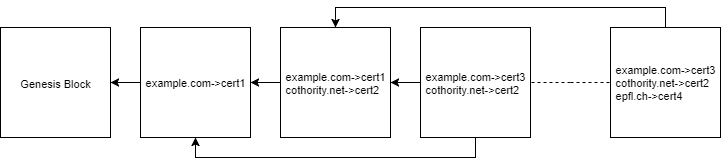
\includegraphics[scale=0.5]{SkipChain.png}
   \caption{SkipChain containing certificates}
\end{figure}
\paragraph{} The idea of the SkipChain is to add other links to every block that points to relatively far away block. Therefore, a user need to get less block to reach the needed one. More precisely, it will need only a logarithmic number of block instead of  a linear one.  
                 
\subsubsection{CISC}
\paragraph{}  Cisc (Cisc Identity SkipChain) is an application in the cothority. It permits to create and manage a personal SkipChain in handled by a cothority. An administrator's device starts a Cisc by connecting to a group of conodes that will handle the SkipChain. The administrator should set up the conodes by sending them his public key. Then, he can run the SkipChain and get an identity number for it. This identity allow other devices to connect to this SkipChain. 
\paragraph{}Cisc maintains a key/value pairs table that the connected devices can modify. They can add, remove and change pairs from it. Any modification cause the creation of a new SkipBlock. Hence, a every block contains a copy of the whole actual table . 
\paragraph{}Cisc establish a system of cryptographic vote. Any modification on a Cisc's table is placed on proposal table and should be submitted to vote to its user. They then have to decide if they want this modification or not. This vote process use a cryptographic protocol named Cosi. It uses the Schnorr signature protocol which permit to combine multiple signature into a single one. Thus, every time a device vote (positively) on a new block he sent his signature to the other one. Therefore, when every devices have voted positively on a new block the signature is complete and it is added to the SkipChain.      
\\In a same way, every connected devices has to vote on the integration of a new device.
\subsection{Related Project}
\subsubsection{Google's Certificate Transparency}
\paragraph{}  Certificate Transparency is a project that also have the goal to prevent miss-issued and malicious certificates and quickly detect them.
The idea is to creates certificates log servers that store records of certificates. The main purpose of those servers is that they are public and therefore anyone can submit or query any certificate log. Hence, everybody has the possibility to control the validity of a certificate.
\begin{figure}[h]
   \centering
   \includegraphics[scale=0.5]{Google_Cert_trans.png}
   \caption{Google Certificate Transparency}
\end{figure}
\paragraph{} The next component of this system is the creation of an application that can control the certificate log of a domain before getting connected. For example, this application could be integrated in web-browser. It can perform two verifications: At first, it checks that the log for the website that the client want to access exist on any of the logs-servers. If it does not exist, the application can prevent the connection or warn the user. Indeed, the absence of the log is suspicious and potentially malicious. The second function is to verify the validity of the log. In the case of an issue, the log needs to explain the reason of it or it risks to be erased.
\paragraph{} The last idea is to integrate monitors that will periodically search for invalid certificates in the certificates' logs. Those monitors can then erase this invalid log and warn the owner of the attached domain about the problem.   

\section{The Project}
\paragraph{} This section will present the project with all its technical aspect using all the building block explain in the introduction.
\subsection{Description}
\paragraph{} To achieve the goal of this project, the certificate manager should be able to perform the following task. As a first requirement, the program should be able to request a TLS certificate from Let's Encrypt Certificate Authority. Then, this new collected certificate needs to be collectively verified to insure its validity. Finally, the certificate will be stored in a SkipChain.
We will use Cisc which, as said before, permits to create and manage a SkipChain. 
The project will contribute to add functionality to this application so that it can support the management of certificates and allow clients to easily use it. The next paragraphs detail the implementation of this addition.
\subsubsection{Request Certificates}
\begin{wrapfigure}{r}{5cm}
   \centering
   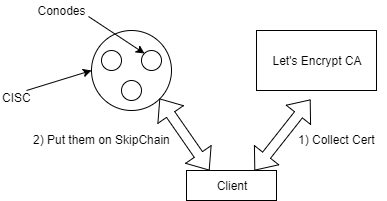
\includegraphics[scale=0.5]{System.png}
   \caption{ Diagram of the system\label{overflow}}
\end{wrapfigure}
\paragraph{} This functionality permits to automatically request a certificate for a given domain from Let's Encrypt CA and store it directly in Cisc.  
Certificates are collected using an ACME client Golang package. At first, the program creates a client for the ACME by querying the Let's Encrypt server resource directory. Then, the program generates a RSA key-pair that is sent to the server to register.
\paragraph{}
As explained earlier, the client needs to complete a challenge which proves to the ACME that he owns this domain before he can request certificates for it. This package supports 3 types of challenge: HTTP-Challenge, TLS-Challenge and DNS-Challenge. At this moment, the code supports only the HTTP-Challenge that is easier to apply for already running servers. To complete it, the client has to store a particular file in a certain domain's directory. The Let's Encrypt server can reach this file by connecting to the site and control that it is the right one. If the challenge is completed, the ACME can safely give certificates to this domain. All the manipulation is made automatically by the request function. The only requirement is that the program needs to be run on the web server so that the challenged file can be created and stored in the right place.       
\paragraph{}
The ACME client still has to create a certificate request that gives some information about the certificate needed,such  as the name of the domain and some other information like the encryption mode and the public key of the future certificate. The program that generates this certificate request sets the minimum information needed. Finally, the client can now request and get the certificate.
\paragraph{}
The new certificate is verified by the program to prevent any security issues. This verification is made by trying to create a chain from the certificate to the Root of Let's Encrypt. If this verification success, the certificate is encoded in a format named PEM (Privacy Enhanced Mail) and stored in the proposed storage of CISC. A new SkipBlock containing the certificate will finally be added to the SkipChain if all the connected device vote positively to the addition of the new certificate. 

The PEM certificate file and its corresponding private key are also stored on the user web server and can be used. The command append automatically the intermediate Let's Encrypt to this file so that every browser can reconstruct the whole certificate chain of trust.
\subsubsection{Renew Certificates}
\paragraph{}This functionality allows a client to renew a certificate already stored on a SkipChain just by passing the name of the domain. This renew functionality allows to extend the expiration date. The ACME client package demands to pass the URI of the certificate to renew it. A copy of every certificate is stored on the ACME web-server and we will pass the URI of this emplacement to the function. Certificates are stored in the ACME using their serial number. So, the URI of a certificate can be computed using this serial number that is unique for every certificate. 
\paragraph{}
If the certificate passed to the function isn't expired, the certificate return is the same. Therefore, if the certificate corresponding on a domain needs to be changed because of a security issues or another reasons the request command should be used. 
\subsubsection{Voting}
As explained earlier, all devices connected to Cisc have to vote positively on a modification in the key/value table before a new SkipBlock can be added on the SkipChain. The project adapts this system to collectively verify certificates. Before making the voting decision, the client can see information about the new or modified certificates. The program verifies the certificate and return the result to the client. Furthermore, if this is a modification of a previous certificate, the program will print the difference between the new and previous so that the client could make a decision about the change.          
\subsubsection{Retrieve Certificates}
\paragraph{}This functionality permits a client to retrieve a certain certificate stored in Cisc. Again, this function check the validity of the certificate and create a PEM encoded file containing the certificate.
\subsubsection{Other Functionality}
\paragraph{Add a certificate}
This functionality allow a client to add a certificate to SkipChain that he gets from another source (without use the Request Certificate function). As before, this function will verify the certificate and add it to the proposal storage. At this moment, the verification support only the Let's encrypt certificate. Indeed, the certificate is compared against the Let's Encrypt Root certificate. Therefore, any other certificate will not pass the verification.
\paragraph{Verify}
This functionality allows a client to verify by himself that a certain certificate stored in Cisc is valid. Its utility is to permit a new client to verify certificates that was yet stored in the SkipChain before its connexion to Cisc.
\paragraph{Revoke}
A certificate can also be revoked by an user and removed from the the SkipChain. Only the ACME account that have request the certificate can revoke it.  

           
\subsection{Limitation}
\paragraph{Number of devices}
The principal security of this protocol repose in the fact that this is hard to hack a lot of devices. Therefore, the number of devices should be big to insure a good protection. This implies that the protocol should be quickly adopted by a certain number of people and this can be hard to perform in practice. Moreover, devices should be as diverse as possible and being connected on different networks to prevent from grouped attacks. Hence, this protocol should be adopted by a lot of institutions (for example CA or company) which could take a long amount of time to perform.
\paragraph{Problem With Voting}
On the current implementation of Cisc, every device should vote on a modification and even this the most secure system it can cause some issues. If some devices are attacked or  unavailable, they may not vote (or vote negatively) to a modification even if this is a legit one. Moreover, for a certain biased point of view or by errors a legit client could decide vote negatively. Therefore even if only one of the devices doesn't vote positively to a modification, the whole SkipChain is blocked and the certificate's table will be quickly out-of-date.
\\Moreover, a client should vote once for all recently change made on a Cisc table. Hence, even if only one of the modification isn't correct, a device should vote negatively to all of them to guaranties the security. So some right changes can't be made.        
\paragraph{Signature}
In this implementation, any client that wants to retrieve a certificate from the SkipChain should necessarily trust that current block in. In fact, even if it's hard a block can be maliciously added to the SkipChain.
As explain earlier, every block is signed by its previous block. Hence, this signature would have to be verified by the client to prevent any security issues. Due to the difficulty to implement this functionality, it wasn't made and can be considered as a future work.
\subsection{Results}
\paragraph{}For testing the implementation of the whole system the goal fixed was to collect, add to the SkipChain, and use a certificate for a particular domain-name. For this end, a web-server was launched and domain-name (cothority.net) was set. 
Firstly, we run three conodes on the web-server and set up a CISC using them. Then, we request a certificate using the new functionality explain earlier. For testing the validity of the certificate and the associate private key, we run the web-server using them and we have been able to verify that accessing cothority.net was secure (using https). To check that the protocol used to collect certificate was correct, we tried to run the request command for "cothority.net" on other devices than its web-server and the command failed because of the uncompleted challenge. This show that the protocol is secure because it avoids any miss-issued certificate to collect using the verification challenge.
\paragraph{} Then, we test that the certificate verification function works correctly. We test some certificate and we have been able to show that certificate delivers from another CA than Let's Encrypt, false certificates, revoked certificates, and out-to-date certificates don't pass the verification function. Moreover, the certificate requested for cothority.net pass it which show that the function works. 
\paragraph{} Finally, we test the whole CISC voting system. For this end, we connected other local user's to the SkipChain containing the cothority.net certificate.  We check that the voting function works for every device and that every device should vote to add a certificate. We then check that the function that shows the difference between two certificate works. 
\subsection{Future Work}
\paragraph{Connection}
As said before, a client that wants to communicate safely with a website should get the certificate from it. A future goal could be that this domain certificate will be stored in a SkipChain and that the client needs to connect to it for getting this certificate. Hence by trusting the SkipChain, the client will be sure the certificate is valid. 
\paragraph{Warning}
Another work could be to create a system that allows the SkipChain to warn a domain owner if someone else tries to store a miss-issued certificate. Furthermore, it can warn the domain if the certificate isn't in the SkipChain and ask him if we want to add it. 
\paragraph{Automatic}    
Finally, it will be great to automate the whole process. If many certificates are added to a SkipChain, their verification will be very hard to be manually. Moreover if every device should vote manually to a modification, the amount of time needed to make a verification will be too big. Hence a future work would be to add a function that could make right decisions.         
\subsection{Conclusion}
\paragraph{}In this project, we spoke about how make the internet more secure and more practical to use. Reinforce the certificate protocol became a necessity with the multiplication of the attack against CA. Hence, use a decentralised protocol may be one of key of those issues. Even if this is relatively easy to implements, deployed it will be a real challenge and can only be accomplished if everyone plays the game.  


\section{User Guide}
\paragraph{}This section will explain clearly how correctly use the Cisc application.  
\subsection{Initialization}
\subsubsection{Requirement}
\paragraph{} At first, notice that you should use a Linux environment to support the implementation of this project.
You need to install the \href{ https://golang.org/doc/install}{golang} language that is the used to implement the project. Then, you need to set up the environment variable
\href{ https://golang.org/doc/code.html#GOPATH}{\$GOPATH} using the command "export GOPATH=goFolder" so that it points to your workspace directory and add GOPATH/bin to PATH 
using command "export PATH=\$PATH:\$GOPATH/bin". Also, you have to install and set up GitHub so that you can download the following package (Using "go get -u" command"):
\begin{itemize}
\item github.com/dedis/cothority/conode
\item github.com/dedis/cothority/cisc
\item github.com/ericchiang/letsencrypt
\end{itemize}
After this, you can now run all of the project. 
\subsubsection{Run conodes}
If you want to run your personal conodes, you should follow these steps:
At first, you need to decide if you want to run it publicly or locally. Public conodes can be reached from outside unlike the local one that are just for testing implementations. The easiest way to run them is to use the bash program "run\_conode.sh" (normally located in \$GOPATH /github.com /dedis/cothority/conode).
This bash will create a directory by running conodes. It contains two files: the public information (public.toml) and the private information (private.toml), this files contain the IP address of the conode and respectively its public and private key. Thus, the private file should not be transmitted to ensure the security of protocols. The bash will also create a group definition file (public.toml) that contain the public informations of all running conodes. 
\subsection{Cisc Commands Overview}
There is seven type of command in Cisc: 
\begin{itemize}
\item Admin: Connect to Conodes and save authentication data
\item Id: Create and manage SkipChain
\item Config: Manage the data of a SkipChain
\item Ssh: Manage the Ssh-data of a SkipChain. 
\item Cert: Manage the certificate table of a SkipChain.
\item Kv: Manage the key/value table (with other content than certificate) of identities
\item Follow: Follow A SkipChain

\end{itemize}
Note that the commands Ssh and Follow are not presented because they are not used.
\\We detail those group of command below:
\paragraph{Admin Command} This command contains those sub-command:
\begin{itemize}
\item Link: establish a connection with a conodes
\item Add: Add a public key on a conode
\item Store: Add authentications data on a conode. We will not use it. 
\end{itemize}
\paragraph{Id}
This command contains those subcommand:
\begin{itemize}
\item Create: Create an Identity SkipChain
\item Connect: Connect to an Existing SkipChain
\item Keypair: generate a public/private keypair  
\end{itemize}
Note that a device can be connected to only one SkipChain.
\paragraph{Config}
This command contains those subcommand:
\begin{itemize}
\item Update: Update the data of the SkipChain 
\item List: Update and list the data of a SkipChain
\item Vote: Vote for a modification in the SkipChain
\end{itemize}
\paragraph{Cert}
This is the newly added command. It contains those subcommand:
\begin{itemize}
\item Request: Request a Certificate and add it on the SkipChain.
\item Add: Add a certificate on the SkipChain table.
\item Renew: Renew a Certificate on the SkipChain Table
\item Verify: Verify a Certificate on the table.
\item List: List the content of the certificate table.
\item Retrieve: Retrieve a Certificate from the table.
\item Revoke: Revoke and delete a Certificate from the table.
\end{itemize}
\paragraph{Kv}
This command is similar to the cert one but should be used with other data than certificate. It contains those subcommand:  
\begin{itemize}
\item List: List the content of the key/value table
\item Add: Add a key/value pairs.
\item Remove: remove a key/value pairs of the table.
\end{itemize}
\subsection{Utilization}
\subsubsection{Run and Set Up Cisc}
In this part we will explain how to run a new Cisc as admin. At first, you need to link your computer to the conodes using the "admin link" command, the utilization of this command implies that you should know conodes IPs. Then, you need to generate a key pair using the “id kp” command and send the public part to the conodes using the "admin store" command. Finally, you can create and run the SkipChain running the "id create" command. This command give you an ID number that will allow other devices to join your SkipChain.
\subsubsection{Connect to an Existing Cisc}
To join a Cisc, you need to pass the group definition (toml file) of the conode handle it and its ID. Knowing this, you can run the command "id connect" that will send a connection request to the SkipChain. All devices already connected have to vote (see section ~\ref{sec:vote}) on your integration before you can be definitely be connected.
\subsubsection{Add a certificate in Cisc}  If you are connected on a Cisc, you can now request Let's Encrypt for your domain and add it to the Cisc. The "cert request" command automatically request the certificate and add it to the proposal storage of Cisc. This command should be run on the domain server so that the HTTP-challenge can be completed. 
The command generate an RSA Key (named registerkey.pem) that should be kept safely and stay secret.Note that the domain has to subscribe to the ACME using an RSA key. The ACME have a maximum threshold of subscriptions for a certain IP address. Therefore, subscribe with many different keys could cause the overtaking of the threshold. Using the same key return the same registration. 

If the challenge is complete, the certificate pass a verification function and is added to the proposal storage of The Cisc. The command also put the certificate (named fullchain.pem) and his private key (named privkey.pem) on your device (In the folder where you run the command). This certificate and its private key can be used to run a secure (https) website.
Note that you can request up to five certificate per week. 
Also, you can add a certificate that you could yet have by using the "cert add" command. 
\subsubsection{Renew a certificate}
A certificate stored on a Cisc can be renewed using the command, "cert renew". This command modify the certificate in the CISC if its expiration date is close or passed. So, a certificate that is still available during a certain amount of time will remain unchanged. Hence, if for some reason you should get a completely new certificate, you need to use the "cert request" command. Note, that the certificate is again verified and put in the proposal storage. 
\subsubsection{Voting}\label{sec:vote} As explain earlier, any change of the SkipChain should be voted to be accepted and incorporated in a new Skipblock. The command "config vote" allow you to vote on the new modification. In the case of a device, the command give you some information about it and it is up to you to decide about is addition.
In the case of a certificate, the command verify for you the certificate and will compare the new certificate with the old entry in case of an update.
\subsubsection{Retrieve a certificate}
You can retrieve a certificate of a certain domain from the SkipChain with the command "cert retrieve" by passing it name. The command verify that the certificate is in the SkipChain and that it's valid. If there are no issues, the certificate (named "domain.pem") is stored in the folder where you run the command.
\begin{thebibliography}{9}

\bibitem{1}
 Ewa Syta, Iulia Tamas, Dylan Visher, David Issac Wolinsky, Bryan Ford, \textit{Certificate Cothority: Towards Trustworthy Collective CAs}
\bibitem{2}
  Ewa Syta, Iulia Tamas, Dylan Visher, David Isaac Wolinsky, Philipp Jovanovic, Linus Gasser, Nicolas Gailly, Ismail Khoffi, Bryan Ford,
  \textit{Keeping Authorities “Honest or Bust”
with Decentralized Witness Co-signing
},
\bibitem{3}
Bryan Ford,\textit{ How do you know it's on the BlockChain? With a SkipChain.},\\\texttt{https://bford.github.io/2017/08/01/skipchain/}
\bibitem{4}
 B. Laurie, A. Langley, E. Kasper, \textit{What is Certificate Transparency?} \\\texttt{https://www.certificate-transparency.org/what-is-ct}
\bibitem{5}
Dedis Lab,\textit{Scalable collective authority prototype},\\\texttt{https://github.com/dedis/cothority}
\bibitem{6}
Eric Chiang, \textit{A Let's Encrypt client for Go}, \texttt{https://github.com/ericchiang/letsencrypt}
\end{thebibliography}


\end{document}


